\subsection{Aufgabenstellung}\label{subsec:aufgabenstellung}
Die vorgegebene Aufgabenstellung 8/9 im Praktikum von Datenbanken und Informationssysteme sieht eine Erstellung und Optimierung eines Java Programms, sowie eines Datenbankmanagementsystem vor.
Hierbei wurde in der vorherigen Aufgabe eine MySQL-Datenbank für die Dateninitialisierung in einer n-tps-Datenbank herangezogen, in der verschiedene Relationen erstellt und anschließend mit Einträgen bzw. Tupeln gefüllt wurden.
Bei dieser Aufgabenstellung sollen nun die erstellten Einträge mittels drei Abfragen / Lasttransaktionen (TXs) in einer 100-tps-Datenbank gelesen und verändert werden.
Die Benchmark-Messungen der Anfragen auf das DBMS erfolgen bei unterschiedlichen Lasten mit verschiedenen Profilen (Last1, Last2, Last3), die durch ein Load-Driver-Programm durchgeführt werden.
\subsection{Datenbankmanagementsystem}\label{subsec:datenbankmanagementsystem-einleitung}
Als Datenbankmanagementsystem wird ein MySQL Server mit der Version 8.0.30 verwendet.
Dieser läuft auf einer virtuellen Maschine, der als Server agiert und durch eine Netzwerkverbindung zum Programm Abfragen / Transaktionen erhält.
Zum lokalen Testen des Programms auf dem eigenen Rechner wird ein Docker-Container mit MySQL Server-Instanz genutzt.
\subsection{Schema / Aufbau der Datenbank}\label{subsec:schema/aufbau}
Das Datenbankschema umfasst vier Relationen.
Diese sind nachfolgend als Abbildung dargestellt, sowie deren Verbindungen durch Fremdschlüssel der jeweiligen Relationen miteinander.
\begin{figure}[h!]
    \center
    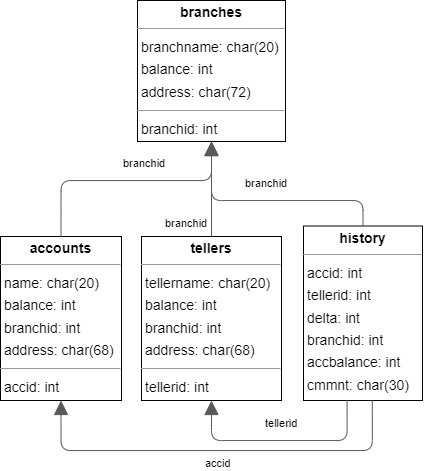
\includegraphics[height=8.5cm]{assets/img/benchmark-datenbank-schema}
    \caption{Benchmark-Datenbankschema}
    \label{fig:benchmark-datenbankschema}
\end{figure}
\subsection{Programme}\label{subsec:programme}
Verwendete Programme bei dieser Aufgabenstellung bezüglich der Erstellung und Optimierung des Java Programms und des Datenbankmanagementsystems sind unter anderen IntelliJ IDEA, MySQL Workbench CE, Data Grip, Docker, sowie der JDBC Treiber (Ver. 8.0.31) für die Schnittstelle/Kommunikation zwischen dem DBMS und dem Java Programm.
\subsection{Lasttransaktionen}\label{subsec:lasttransaktionen}
Nachfolgend werden die drei Abfragen / Lasttransaktionen (TXs) im Detail beschrieben.
Diese sollen die bekannten ACID-Eigenschaften garantieren und werden nach einer relativen Gewichtung von 35 zu 50 zu 15 für Kontostands-, Einzahlungs- und Analyse-TX im Load-Driver-Programm ausgeführt.
\begin{enumerate}
    \item \textbf{Kontostands-TX} \\
    Eine Methode, die einen Kontostand (balance) zu der zugehörigen Kontonummer (accid) abfragt und als Rückgabewert liefert.
    \item \textbf{Einzahlungs-TX} \\
    Eine Methode / Abfrage, die als Einzahlung eines Betrages agiert und eine Kontonummer (accid), Geldautomatennummer (tellerid), Zweigstellennummer (branchid) und eine Einzahlungsbetrag (delta) als Eingabeparamter erwartet.
    In dieser Transaktion werden Einzelaktionen durchgeführt, wie das Aktualisieren der Bilanzsumme (balance) zu den zugehörigen Nummern (accid, branchid, tellerid) in den verschiedenen Relationen (accounts, branches, tellers).
    Des Weiterem das Erstellen einer Einzahlung als Beleg in der Relation history mit den zugehörigen Nummern (accid, branchid, tellerid), den Einzahlungsbetrag (delta), den aktualisierten Betrag (accbalance) von der Relation accounts, sowie einen Kommentar (cmmnt).
    Als Rückgabewert wird der aktualisierte Betrag (accblance) von der Relation accounts zurückgeben.
    \item \textbf{Analyse-TX} \\
    Eine Methode / Abfrage zur Rückgabe der Anzahl der getätigten Einzahlugen mit genau einem Betrags (delta), der als Eingabeparameter übergeben wird.
\end{enumerate}

\subsection{Load-Driver-Programm}\label{subsec:load-driver-programm}
Das Load-Driver-Programm dient zu Messung / Benchmark des DBMS und führt dabei 10 Minuten lang eine Schleife aus, wobei es eine 4-minütige Einschwingphase, dann eine 5-minütige Messphase und am Ende eine 1-minütige Ausschwingphase gibt.
In der Schleife werden dann durch die relative Gewichtung der Lasttransaktionen, diese zufällig gewählt und mit zufällig gewählten, sinnvollen Parametern ausgeführt.
Die Primary Keys oder Fremdschlüssel der Einträge (accid, branchid, tellerid) werden dabei zufällig und gleichverteilt aus den jeweiligen Bereichen gewählt.
Die Einzahlungsbeiträge werden zufällig und ebenfalls gleichverteilt aus dem Bereich 1 bis 10.000 erzeugt.
Außerdem soll  zwischen zwei TXs jeweils eine feste Nachdenkzeit / Pause von genau 50 ms eingehalten werden, sodass das Programm nach erfolgreicher Abarbeitung einer TX einfach wartet, bevor die nächste gestartet wird.